\chapter{Related Work}\label{chap:relatedwork}
Citation recommendation as a field has been around for quite some time. But as Figure~\ref{fig:citationyears} shows, it took some time before it became popular. McNee~\cite{McNeeACGLRKR02} was probably the first to delve into this field -- a global recommendation system was explained in this paper from 2002. There was a gap of 5 years before research into citation recommendation systems continued with Strohman et al.~\cite{StrohmanCJ07}, which describes another two-stage global citation recommender system. Since then, there have been a multitude of papers about both global and local citation recommendation.
\begin{figure}[h]
    \centering
    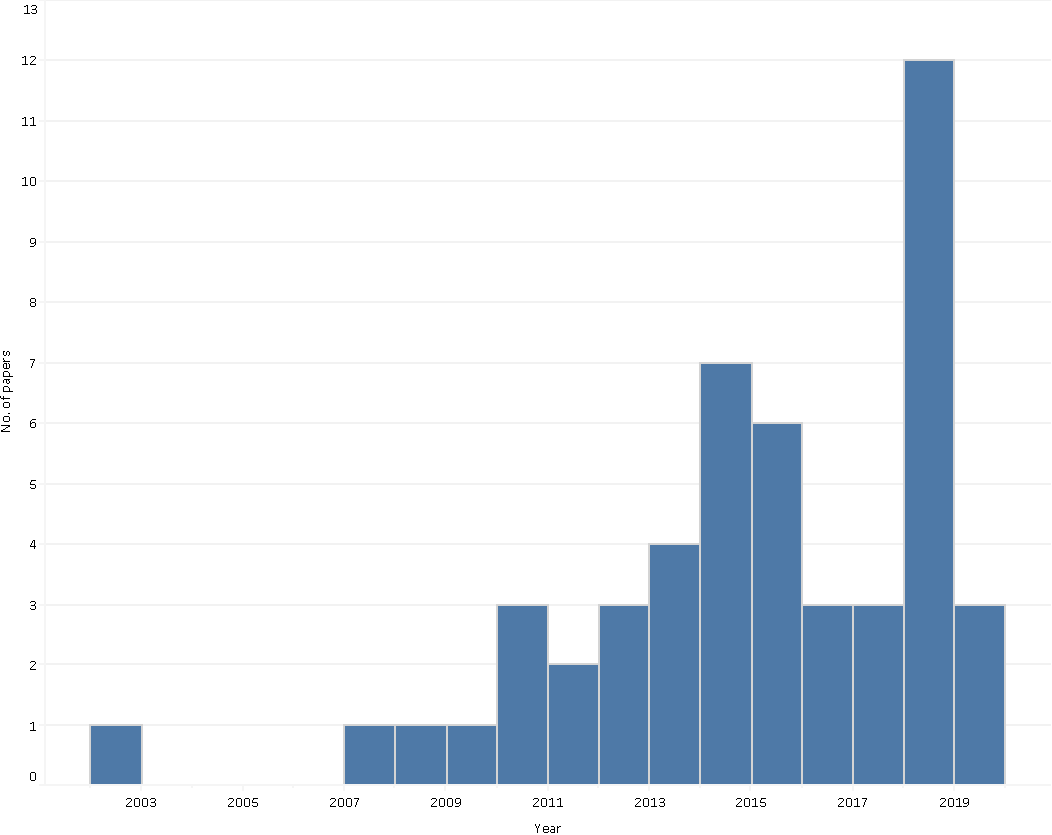
\includegraphics[width=10cm]{figures/yearcitations.pdf}
    \caption{Popularity of Citation recommendation as a field (based on no. of papers published)}
    \label{fig:citationyears}
\end{figure}
\section{Local Citation Recommendation}
The term 'context-aware' recommendation only came into being in 2010 with the seminal He et al. paper~\cite{He2010}. This was the first paper which covered local recommendation (alongside global or context-oblivious recommendation). The same authors followed up this study with a statistical machine translation model in~\cite{He2011}. This idea of using a machine translation model is then taken forward to Huang et al, 2012~\cite{HuangKCMGR12}, where they use the idea that specific keywords in the contexts (source language) are translated to cited documents (target language). Their system, in essence, is a de-facto machine translation system for citation recommendation. 
\section{Embedding-based Approaches}
Embeddings are low-dimensional representations of high-dimensional vectors. 
Mikolov et al~\cite{MikolovSCCD13} was the famous paper that introduced Word2Vec, which is a method of converting words into fixed low-dimensional vectors. This led to the paper by Le and Mikolov~\cite{LeM14}, which extended word vectors to paragraph vectors which could be computed for a set of words or an entire document. 
Paragraph vectors were combined with a graph-based random walk method called DeepWalk (Perozzi et al.~\cite{PerozziAS14}) in Ganguly et al.~\cite{GangulyP17}, which is covered in much more detail in Chapter 5. The aim of this paper was not for citation recommendation, but rather for node classification and link prediction. However, we adapt it for citation recommendation in chapter 5. 

There have been a number of embedding-based approaches in the citation recommendation field. The first one was probably Tang et al, 2014~\cite{TangWZ14}, which used TF-IDF vectors to construct cross-language embeddings for local citation recommendation. Jiang et al.'s two papers (\cite{JiangLL18,JiangYGLL18}) also use embeddings in the context of cross-language citation recommendation, but in the global recommendation area. Cai et al, 2018~\cite{CaiHY18} and Zhang et al, 2018 \cite{ZhangYCD18} (which uses paragraph vectors) are also embedding-based global citation recommendation approaches.

Moving back to local citation recommendation embedding approaches, Huang et al, 2015~\cite{Huang2015} was one of the follow-up papers to Huang et al, 2012~\cite{HuangKCMGR12}. Here, they continue their focus on translation models, but add in distributed word representations of the words and cited documents in the citation contexts (Mikolov et al~\cite{MikolovSCCD13}). 

The Hyperdoc2vec paper~\cite{ShiSZZH18} is one of the most recent papers which use embedding-based neural networks. In this paper, the authors aim to learn two representations of each document -- one by treating it as a citing document and the other by treating it as a cited document. They use the full text of the citing and cited documents and claim that their method works better according to four criteria: content awareness, context awareness, newcomer friendliness, and context intent awareness. This approach is adapted in this thesis due to these features. It will be covered in detail in Chapter 5. 
\section{Topic Modelling, Information Retrieval and Random Walks}
Topic modelling and in particular LDA~\cite{BleiNJ03} have been used in multiple citation recommendation papers (\cite{KatariaMB10, DBLP:Jiang13, NallapatiAXC08, LiuYGSG14}). In this thesis, we use LDA as a baseline.

Information retrieval techniques have also been used in previous papers, from TF-IDF-based text comparison, to BM25. Duma et al's two papers (\cite{DumaKLRC16, DumaLCRK16}) both treat citation recommendation as an information retrieval task, while a few papers like Ebesu et al.~\cite{Ebesu2017} use BM25 as a simple baseline. BM25 plays an important role in the hybrid recommendation system created in this thesis. 

Random walks through a citation graph are used in multiple papers (\cite{JiangLL18, JiangYGLL18, CaiHY18, ChakrabortyMNN15} among others). We use random walks to enrich paragraph vectors in the Paper2Vec approach.
Random walks, LDA and BM25 are explained in more detail in Chapter 3, and used in Chapter 5.

One set of algorithms which we won't cover in this thesis go by the name of \textit{personalised citation recommendation} algorithms. These are algorithms which include the author details and other information such as details of the venue/conference, and use them to get personalised recommendations. These tend to perform better, but there is a degree of bias introduced, and it also requires these details to be provided during the prediction phase. 
These personalised algorithms are common in other types of recommender systems, but Liu et al.~\cite{LiuYY13} was probably one of the first to implement a personalised algorithm for citation recommendation. There have been multiple other personalised approaches based on deep learning recently, including Ebesu et al.~\cite{Ebesu2017} (which includes author information), Yang et al.~\cite{YangZCDMGD18} (which includes venue and author information), Cai et al, 2018~\cite{CaiHY18} and Zhang et al, 2017.~\cite{Zhang2017}
\section{Hybrid recommender systems}
It would be expedient to mention hybrid recommender systems at this point of time. Burke \cite{Burke2002, Burke2007} provides an excellent introduction/survey about hybrid recommender systems. Hybrid recommender systems are systems which take predictions from two or more disparate recommender systems, and combine them in different ways. The famous example for hybrid recommendations is that of combining a collabarative-filtering based recommender and a content-based recommender. 
There are a myriad of ways in which recommendations of two systems can be combined according to Burke~\cite{Burke2002}: weighted, switching, mixed, feature combination, cascade, feature augmentation and meta-level. 

In the citation recommendation context, Hsiao et al.\cite{HsiaoCD15} use a hybrid recommendation system which combines results from two disparate systems.
A two-step process (candidate generation, ranking) to citation recommendation is followed in several papers including Zarrinkalam~\cite{Zarrinkalam2013}, Rokach et al.~\cite{Rokach2013}, Bhagavatula et al.~\cite{Bhagavatula2018} and McNee~\cite{McNeeACGLRKR02}, but these aren't hybrid systems per se -- they only use two different algorithms for candidate generation and ranking.
A hybrid citation recommendation system is built as part of this thesis and is explained in Chapter 5.